%
% Annual Cognitive Science Conference
% Sample LaTeX Paper -- Proceedings Format
%

% Original : Ashwin Ram (ashwin@cc.gatech.edu)       04/01/1994
% Modified : Johanna Moore (jmoore@cs.pitt.edu)      03/17/1995
% Modified : David Noelle (noelle@ucsd.edu)          03/15/1996
% Modified : Pat Langley (langley@cs.stanford.edu)   01/26/1997
% Latex2e corrections by Ramin Charles Nakisa        01/28/1997
% Modified : Tina Eliassi-Rad (eliassi@cs.wisc.edu)  01/31/1998
% Modified : Trisha Yannuzzi (trisha@ircs.upenn.edu) 12/28/1999 (in process)
% Modified : Mary Ellen Foster (M.E.Foster@ed.ac.uk) 12/11/2000
% Modified : Ken Forbus                              01/23/2004
% Modified : Eli M. Silk (esilk@pitt.edu)            05/24/2005
% Modified : Niels Taatgen (taatgen@cmu.edu)         10/24/2006
% Modified : David Noelle (dnoelle@ucmerced.edu)     11/19/2014
% Modified : Roger Levy (rplevy@mit.edu)     12/31/2018



%% Change "letterpaper" in the following line to "a4paper" if you must.

\documentclass[10pt,letterpaper]{article}

\usepackage{cogsci}

%\cogscifinalcopy % Uncomment this line for the final submission


\usepackage{pslatex}
\usepackage{apacite}
\usepackage{enumitem}
\setlist{noitemsep,topsep=0pt,parsep=0pt,partopsep=0pt,leftmargin=*}
\usepackage{graphicx}
\usepackage{dblfloatfix}
\usepackage{float} % Roger Levy added this and changed figure/table
                   % placement to [H] for conformity to Word template,
                   % though floating tables and figures to top is
                   % still generally recommended!

%\usepackage[none]{hyphenat} % Sometimes it can be useful to turn off
%hyphenation for purposes such as spell checking of the resulting
%PDF.  Uncomment this block to turn off hyphenation.


%\setlength\titlebox{4.5cm}
% You can expand the titlebox if you need extra space
% to show all the authors. Please do not make the titlebox
% smaller than 4.5cm (the original size).
%%If you do, we reserve the right to require you to change it back in
%%the camera-ready version, which could interfere with the timely
%%appearance of your paper in the Proceedings.



\title{Color semantics in language predict color associations in blind and sighted individuals.}

\author{{\large \bf Jeroen van Paridon (vanparidon@wisc.edu)} \\
  Department of Psychology, 1202 W. Johnson Street \\
  Madison, WI 53706 USA
  \AND {\large \bf Ella Qiawen Liu (qliu295@wisc.edu)} \\
  Department of Psychology, 1202 W. Johnson Street \\
  Madison, WI 53706 USA
  \AND {\large \bf Gary Lupyan (lupyan@wisc.edu)} \\
  Department of Psychology, 1202 W. Johnson Street \\
  Madison, WI 53706 USA}


\begin{document}

\maketitle


\begin{abstract}
Colors are strongly associated with certain semantic dimensions (e.g. red is hot, blue is cold). Many of these associations are grounded in our visual perception of the world around us, but blind people can reproduce some of these associations, which suggests color semantics can also be learned from language. How are these color semantics represented in written and spoken language? And how does our use of language align color semantics between individuals?
We apply a projection method to word embeddings trained on large corpora of spoken and written text to identify color-semantic associations represented in language. We show that these projections are predictive of color-semantic ratings collected from blind and sighted individuals, but that the effect size varies with embedding training corpus. Finally, we examine how color-semantic associations might be represented in language by training word embeddings on corpora from which various sources of color-semantic information are removed.

\textbf{Keywords:}
language; semantic features; distributional semantics
\end{abstract}

\section{Introduction}
Much of what we know about the world we learn by perceiving and interacting with it, and consequently we often talk about knowledge as if it can only be acquired through personal experience. This has sometimes led to the presumption that people who lack certain experiences (e.g. because they are blind or deaf) do not understand the nature of these experiences. It was long thought, for instance, that blind people could not understand the concept of color (both John Locke and David Hume were of this opinion). Evidence from behavioral studies, however, suggests that blind participants can in fact distinguish between cool and warm colors \cite{shepard1992representation} and that some are able to rate color similarities with enough accuracy that multidimensional scaling of the pairwise similarities yields an arrangement that resembles the color wheel \cite{marmor1978age,saysani2018colour}. Most recently, \citeA{saysani2021seeing} collected semantic differential ratings for color words from both blind and sighted individuals and used multidimensional scaling to demonstrate that there is considerable variability between blind individuals and that some, but not all, blind participants generate semantic differentials that are highly similar to the ones generated by sighted people. Since blind participants have no means of directly perceiving color associations, it perhaps seems obvious that they learn color-semantic knowledge from language. \emph{How} color-semantic information is represented in spoken and written language--and to what extent language, rather than visual perception, aligns color semantics between individuals--is, however, not obvious. Are color semantics conveyed explicitly? Are they conveyed through simple cooccurrences? Or are color semantics encoded in more complex semantic structures--a web of associations that we can derive color semantics from?

We conduct four experiments to further explore these questions: In Experiment 1 we reanalyze data collected by \citeA{saysani2021seeing} using word embeddings (a class of distributional semantics model) to get a quantitative measure of the relationship between participants' color-semantic differential ratings and the color semantics represented in language. In Experiment 2 we replicate our findings from Experiment 1 in a sighted sample, but we also explore whether participants perceive their own color semantics as differing from those of others. In Experiment 3 we replicate our findings in yet another, larger, sighted sample, and also explore whether more exposure to certain kinds of language causes participants' color semantics to be more aligned. In Experiment 4, we test several hypothesized origins of color-semantic information in word embeddings by selectively removing them from the corpus the embeddings are trained on.

\section{Experiment 1: Reanalysis of \citeA{saysani2021seeing}}
\subsection{Word Embedding Projections}
Using word embeddings, we draw an axis from one end of a semantic dimension (e.g. \emph{hot}) to the other end (e.g. \emph{cold}) and then project the word embedding for each color onto that axis (see \citeNP{grand2018semantic} for a discussion of this projection method, but note the method we use here differs slightly in that we normalize the semantic axes before projecting the color embeddings). This provides us with a \emph{relative} measure of word similarity, taken along the semantic dimension's axis, that we can use to predict human ratings of color associations.

Word embeddings are trained on large text corpora, and as such the semantic information they capture tends to reflect the contents of the corpus they are trained on. Using the projection method, we computed color associations in embeddings trained on four different text corpora: The Common Crawl and Wikipedia \cite{grave2018learning}, the OpenSubtitles corpus \cite{van2020subs2vec}, and the subcorpora of the Corpus of Contemporary American English (COCA; subcorpora are fiction, news, academic texts, spoken texts, and magazine articles).

\section{Method}

\subsection{Participants}
\citeauthor{saysani2021seeing} recruited 32 participants, 20 of whom had normal, trichromatic vision. The remaining 12 were congenitally blind, with no residual experience of vision.
\subsection{Design and Procedure}
Participants were asked to rate each of nine color terms (red, orange, yellow, green, blue, brown, purple, black, and white) on 17 semantic dimensions, each defined by two antonyms placed at the poles of a seven-point Likert scale (happy–sad, calm–angry, submissive–aggressive, relaxed–tense, exciting–dull, selfless–jealous, active–passive, like–dislike, alive–dead, fast–slow, new–old, unripe–ripe, soft–hard, light–heavy, fresh–stale, clean–dirty, and cold–hot).
\section{Results}
The main finding reported by \citeA{saysani2021seeing} was that multidimensional scaling solutions were more variable between blind participants than between sighted participants. Comparing intraclass correlations for the blind (.35, 95\% CI [.29, .42]) and the sighted (.49, 95\% CI [.43, .55]) groups also suggests the blind participants are more variable than the sighted participants. Between-participant variability does not mean however that there is no common variance in individual participants' scores that can be predicted from a common measure.

Using a Bayesian linear mixed-effects model with weakly regularizing priors \cite{yarkoni2016bambi}, we regress word embedding projections onto participants' color-semantic association ratings, while adjusting for dimension word frequency, dimension word concreteness, and how often a given color was provided as response to cueing with a given semantic dimension pole word in the Small World of Words dataset \cite<SWOW;>{de2019small}. The model accounts for random variability by including participant-, color-, and dimension-level random intercepts but also participant-level random slopes for embedding projections, SWOW labels, dimension word frequency and dimension word concreteness, as well as colors and dimensions (see online supplementary materials for more information about model structure).

Both the SWOW differential scores and the word embedding projections have predictive value for the participants' color-semantic ratings. SWOW differential scores have an estimated standardized effect size of -.25 (95\% CI [-.29, -.21]); word embedding projections have an estimated standardized effect size of -.58 (95\% CI [-.66, -.50]) in sighted participants and -.37 (95\% CI [-.48, -.26]) in blind participants when trained on COCA-fiction, but the effect size estimates are smaller for embeddings trained on other corpora, with COCA-spoken performing worst (see Figure 1 for effect size estimates).

\begin{figure}[h!]
\begin{center}
\fbox{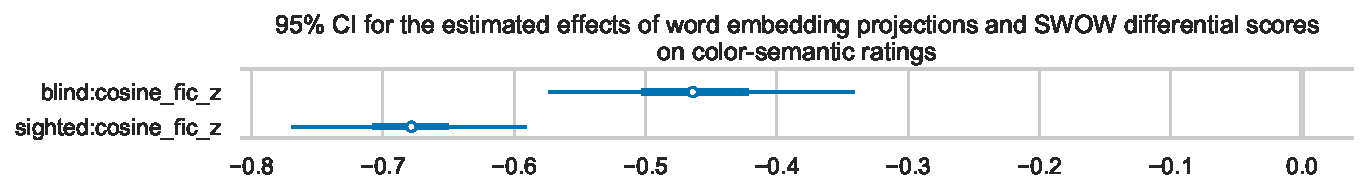
\includegraphics[width=\columnwidth]{figures/original_fiction_forest.pdf}}
\caption{Estimated effects of word embedding projections from various corpora in predicting sighted participants' color-semantic ratings. (Circles are mean estimated effect size, bars represent 95\% CIs.)}
\label{original}
\end{center}
\end{figure}

\section{Discussion}
Color-semantic associations in language may arise from our visual perception of the world around us, but they appear to be predictive for both blind and sighted participants' ratings of color semantics. This suggests that even though blind participants are more variable in their color semantics, they learn color semantics from language, aligning their color semantics with those of sighted people.

\subsection{Differences between word embedding training corpora}
Each of the corpora we used yielded color associations that were predictive of the human ratings of color associations, but the corpus that yielded the most predictive associations (i.e. the largest effect size) was the fiction subcorpus of the Corpus of Contemporary American English (COCA-fiction). There are various possible reasons why the fiction subcorpus, specifically, would render a high quality representation of color associations: The fiction subcorpus is relatively high in quality (wide ranging semantic scope, long and coherent sentences, etc.), compared to e.g. the news corpus (which is more limited in semantic scope and contains many short sentences) or the spoken subcorpus (which largely consists of talk radio interviews, etc.). However, what is likely most important is that fiction contains many idiomatic expressions that convey (or are even the primary source of) color associations, such as stating someone is turning blue (when they are cold), green (with jealousy), or red (with anger or embarrassment). These idioms are less common (or absent) in news and academic texts, and may be less consistently (or intelligibly) used in spoken text of the sort that is included in the COCA-spoken subcorpus.

\subsection{Between-participants variability and self- versus other-ratings}
That we are able to use word embeddings to predict some of the variability in participants' color-semantic ratings suggests that they are at least partly informed by a common understanding of color-semantics (a common understanding which is also represented to some extent in the language of large text corpora). Not all variability in participant ratings is predicted by word embeddings however, and the intraclass correlations between participants suggest that there is a considerable amount of variability between participants. Some of this variability may be due to sampling error, but another source of variability could be that participants' color semantics are idiosyncratic, shaped by experiences unique to each individual (e.g. you might think calm is associated with the color yellow because the yoga studio you go to has yellow walls).


\section{Experiment 2: Replication of sighted results}
To test whether participants \emph{perceived their own} color-semantic associations as idiosyncratic, we conducted a replication of Experiment 1 with sighted participants, whom we asked to provide not only color-semantic ratings for themselves (\emph{self-ratings}), but also their expectation of color-semantic ratings other participants would provide (\emph{other-ratings}).
\section{Method}
\subsection{Participants}
We recruited 30 undergraduate psychology students from the student participant pool at a large research university.
\subsection{Design and Procedure}
Stimuli and procedure were identical to those used in Experiment 1, with two exceptions:
\begin{enumerate}
\item The experiment was carried out online rather than in person.
\item We asked participants to provide not only their own color-semantic association ratings, but also the color-semantic associations they expected others to provide.
\end{enumerate}

\section{Results}
Using the model structure described in Experiment 1, with the addition of a binary variable describing whether a rating is a self- or an other-rating (and interactions between that variable and the various other variables), we again regress word embedding projections and SWOW differential scores onto participants' color-semantic association ratings.

Self- and other-ratings provided by participants were almost perfectly correlated (Pearson r = .98). Bayesian linear mixed effects modeling showed no difference in self- versus other-ratings (mean estimated effect size .00, 95\% CI [-.03, .04]) and embedding projections nor SWOW differential scores were equally predictive of self- and other-ratings (mean estimated interaction for embedding projections and self- vs. other-ratings .01, 95\% CI [-.01, .03], mean estimated interaction for SWOW differential scores and self- vs. other-ratings .00, 95\% CI [-.02, .02]), for marginal effect sizes in self- and other-ratings see Figure 2.

\begin{figure}[h!]
\begin{center}
\fbox{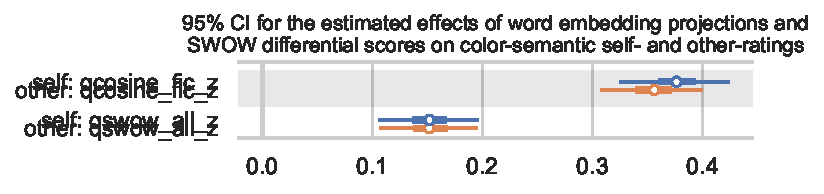
\includegraphics[width=\columnwidth]{figures/self_other_forest.pdf}}
\caption{Estimated effects of word embedding projections and SWOW differential scores in predicting sighted participants' color-semantic self-ratings and other-ratings. There is no meaningful difference between self- and other-ratings. (Circles are mean estimated effect size, bars represent 95\% CIs.)}
\label{self_other}
\end{center}
\end{figure}

\section{Discussion}
While some color-semantic associations \emph{may} be idiosyncratic, participants certainly do not perceive their own associations as differing from others'.



\section{Experiment 3: Associating reading measures with fiction-like color semantics}
\section{Method}
\subsection{Participants}
We recruited 100 undergraduate psychology students from the student participant pool at a large research university.
\subsection{Design and Procedure}
Stimuli and procedure were identical to those used in Experiment 1, with two exceptions:
\begin{enumerate}
\item The experiment was carried out online rather than in person.
\item We asked participants how many hours per week they spend reading fiction and nonfiction text, and had them complete the Author Recognition Test \cite<ART;>{stanovich1989exposure}. The ART is meant to assess a participant's exposure to the names of prominent authors and is predictive various other reading-related measures.
\end{enumerate}

\section{Results}
We analyzed this experiment using the model described in Experiment 1, with added predictors for the reading measures and their interaction with the word embedding projections from the COCA-fiction corpus.
None of the reading measures interact with the word embeddings projections in predicting color-semantic ratings (see Figure 3 for estimated effect sizes).
\begin{figure}[h!]
\begin{center}
\fbox{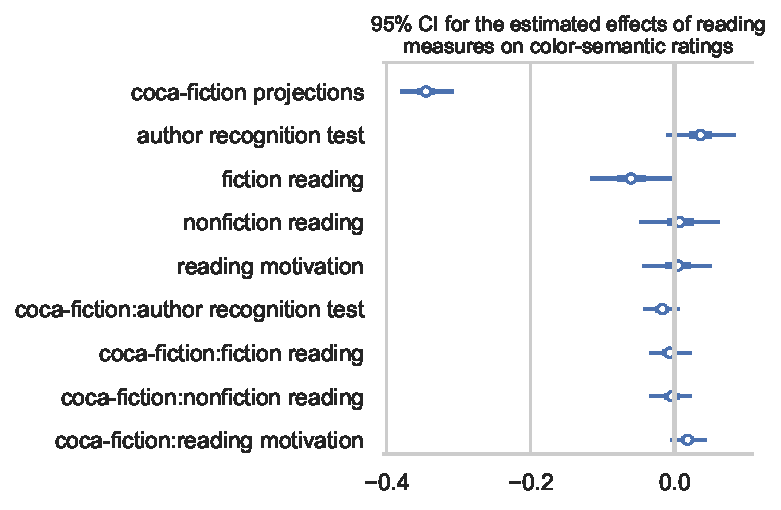
\includegraphics[width=\columnwidth]{figures/reading_measures_forest.pdf}}
\caption{Estimated effects of word embedding projections, various reading measures, and the interactions between projections and reading measures in predicting sighted participants' color-semantic ratings. The predictiveness of fiction-derived word embedding projections does not appear to be higher for participants with more reading exposure. (Circles are mean estimated effect size, bars represent 95\% CIs.)}
\label{reading_measures}
\end{center}
\end{figure}

\section{Discussion}
Given the predictive power of the COCA-fiction word embedding projections (relative to those based on spoken text or Wikipedia/Common Crawl), it is somewhat surprising that reading more fiction does not cause participants to be more aligned with the word embedding projections. However, it is possible that since our participants are all undergraduate students at a large research university, their shared linguistic and cultural background (reading the same books in school, watching the same tv shows growing up, using the same social media) could mean they are already strongly semantically aligned, essentially creating a ceiling effect that obscures any alignment due to additional exposure to written fiction.

\subsection{Meta-analytic effect size of embedding projections in predicting color semantics}
When we pool data from all three experiments, we can obtain a better estimate of the effect size of embedding projections in predicting the color-semantic ratings of sighted participants. [Insert meta-analytic effect size and discussion?]

\subsection{Where do the embeddings ``learn'' their color semantics?}
One potential way of finding the source of these color associations (in the word embeddings, at least) is to try to modify the training corpus in such a way that the associations disappear from the embeddings (and the projected associations are no longer predictive of human ratings). If we can identify the sentences in the training corpus that give rise to the color associations, can these sentences tell us whether (and how) humans learn color associations from language?

\section{Experiment 4: Identifying sources of color-semantic information in embedding training corpora}
Identifying the sentences that are most informative for color associations in a training corpus is not a trivial problem: there is a computational cost to training word embeddings, so performing an exhaustive search is not feasible. Nevertheless, we can start by testing several "naive" hypotheses:
\begin{enumerate}[label=(\alph*)]
\item Color associations are driven by \emph{first-order} cooccurrences, the occurrence of a color word and a semantic dimension word in the same sentence (e.g. "the fire was \emph{red hot}"; color associations in these sentences \emph{can} be explicit, but often are not).
\item Color associations are driven by \emph{second-order} cooccurrences, the occurrence of color words and semantic dimension words in similar contexts (i.e. color words and semantic dimension words may not cooccur, but the share words that they cooccur with, e.g. "Southern cooking uses \emph{green} tomatoes" and "Southern cooking uses \emph{unripe} tomatoes").
\item Color associations are driven by cooccurrences between color words and words in the same semantic neighborhood as semantic dimension words (e.g. "The forest was \emph{white} with \emph{snow}", snow being in the same semantic neighborhood as \emph{cold}).
\item Less direct semantic associations that happen to be very salient. We do not expect these to be represented in the training data in a specific form, but their salience means we should be able to easily elicit them from human participants.
\end{enumerate}
These sources of color-semantic information need not be mutually exclusive; words captured by (c) and (d) may overlap, and all of these words may be part of the set of word described by (b).

\section{Methods}

\subsection{Participants}
We recruited 100 undergraduate psychology students from the student participant pool a large research university to provide labels associated with color-semantic dimensions.
\subsection{Design and Procedure}
For the first-order cooccurrence hypothesis, we removed from the COCA-fiction corpus any sentence containing both a color word and one of our semantic dimension words. For the semantic neighborhood hypothesis, we removed from the COCA-fiction corpus any sentence containing one of the 10 nearest neighbors of each semantic dimension word. The second-order cooccurrence hypothesis proved to be difficult to test: The number of sentences containing shared words is vastly larger than the number of sentences containing first-order cooccurrences, so indiscriminately removing all of these shared words (and the sentences they occur in) reduces the size of the training corpus by an order of magnitude, making it infeasible to test this hypothesis without narrowing down which shared words are most informative for the color-semantic associations.but this reduced the size of the corpus by an order of magnitude, making it impossible to properly contrast embeddings trained on this filtered corpus with the original COCA-fiction embeddings.

For the indirect links through salient words hypothesis, we collected labels for color-semantic associations. Participants were presented with a prompt asking them to provide a label for the pairing of a color and one of the semantic dimension words used in Experiments 1-3 (e.g. "What word comes to mind for \emph{white} and \emph{cold}?"), this was repeated for each of three colors and 34 dimension words, for a total of 102 trials per participant (color groupings were counterbalanced across participants so that all nine colors were presented an equal number of times). We computed name agreement and Simpson's diversity \cite{simpson1949measurement} for the labels participants provided for each color/semantic dimension word pair. We then removed from the COCA-fiction corpus any sentence containing a label provided by at least two participants before training word embeddings on the corpus.

\section{Results}
Removing first-order cooccurrences did not meaningfully reduce the effect size of the COCA-fiction word embedding predictions. Removing nearest neighbors and especially removing participant-generated labels for color-semantic associations had a measurable impact however (see Figure 4 for estimated effect sizes).

\begin{figure}[h!]
\begin{center}
\fbox{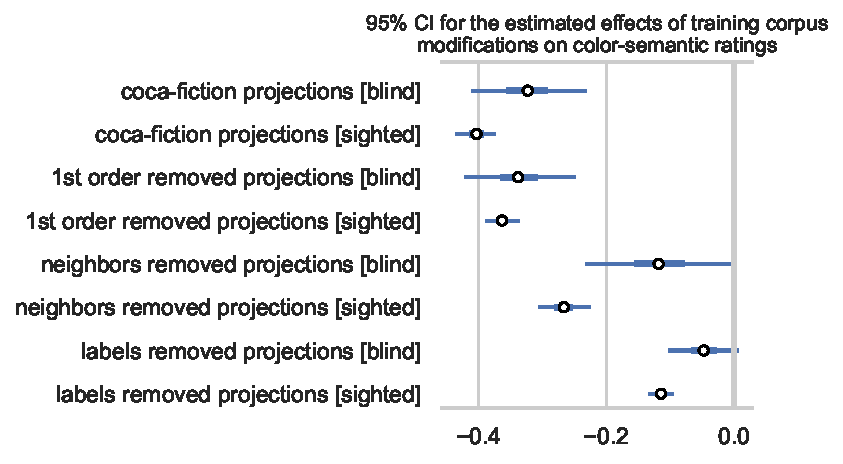
\includegraphics[width=\columnwidth]{figures/corpus_modification_forest.pdf}}
\caption{Estimated effects of word embedding projections in predicting blind and sighted participants' color-semantic ratings. (Circles are mean estimated effect size, bars represent 95\% CIs.)}
\label{corpus_modification}
\end{center}
\end{figure}

\section{Discussion}
That removing first-order cooccurrences had no measurable effect is perhaps not surprising: The objective use to train word embedding models is to predict the context a word occurs in. Strict first-order cooccurrence therefore does nothing to drive embedding similarity. That removing participant-generated labels for color-semantic associations is so effective in removing color-semantic information from the embedding projections is striking, since the number of labels generated by at least two participants (the threshold for inclusion in our corpus filtering procedure) was only about 300 words. Future work will explore whether these labels also satisfy the second-order cooccurrence hypothesis, or if the semantic structures that underpin color-semantic associations arise from still higher-order cooccurrence patterns.

\section{Acknowledgments}
We would like to thank Armin Saysani and Michael and Paul Corballis for making available the raw data we reanalyzed in Experiment 1.

\bibliographystyle{apacite}

\setlength{\bibleftmargin}{.125in}
\setlength{\bibindent}{-\bibleftmargin}

\bibliography{color_semantics}


\end{document}
